\documentclass{article} % For LaTeX2e
\usepackage{nips14submit_e,times}
\usepackage{hyperref}
\usepackage{url}
\usepackage{graphicx}
%\documentstyle[nips14submit_09,times,art10]{article} % For LaTeX 2.09


\title{SSL via Locally Sensitive Hashing (LSH)}


\author{
Timothée Lacroix \\
MVA student - ENS Cachan\\
\texttt{timothee.lacroix@ens.fr} \\
\And
Judith Abécassis \\
MVA student - ENS Cachan \\
\texttt{judith.abecassis@ens.fr} \\
}

% The \author macro works with any number of authors. There are two commands
% used to separate the names and addresses of multiple authors: \And and \AND.
%
% Using \And between authors leaves it to \LaTeX{} to determine where to break
% the lines. Using \AND forces a linebreak at that point. So, if \LaTeX{}
% puts 3 of 4 authors names on the first line, and the last on the second
% line, try using \AND instead of \And before the third author name.

\newcommand{\fix}{\marginpar{FIX}}
\newcommand{\new}{\marginpar{NEW}}

%\nipsfinalcopy % Uncomment for camera-ready version

\begin{document}


\maketitle

\begin{abstract}
Several Semi-Supervised Learning algorithms make use of unlabeled examples to estimate a manifold through a discrete graph that represents it well. Building a complete and exact graph is a $O(n^2)$ operation, which is intractable for larger scale problems. A sensible way of dealing with this issue is to use approximate nearest neighbors search to find the edges of a k-NN (hence sparse) graph. Using Locally Sensitive Hashing will lead to some errors in the graph construction. This article is a study of how those errors will affect the generalization bound on the Harmonic Function Solution for label propagation on a graph. Practical results on the CIFAR dataset will complement those theoretical results.
\end{abstract}


\section{Introduction}
In this work, we are interested in semi-supervised learning (SSL) settings on a large number of points. Such efficient methods can scale and deal with raw data directly collected from the internet and without further filtering. As an example of such a dataset, we can consider the classification of images. A first problem is to extract relevant features, and another problem, which is our focus here, is to efficiently classify unlabeled images using a small number of labeled examples - i.e. SSL. SSL methods often rely on the density structure of the data itself to propagate known labels to areas lacking annotations, and provide a natural way to incorporate labeling uncertainty. However, to model the density of the data, each point must measure its proximity to every other. This requires polynomial time – prohibitive for large-scale problems. 

 The most popular approaches are based on the graph Laplacian, which do not scale for two distinct reasons (we consider $N$ nodes):
\begin{itemize}
\item the construction of the graph itself requires $N^2$ distance comparisons,
\item the manipulation of the laplacian matrix itself (inversion is not possible etc).
\end{itemize}

Previous work (citer Fergus) has previously tackled this issue by only considering the first eigenvalues of the Laplacian, and compute the approximation without needing to consider the full matrix. To achieve this goal, the authors apply results from the spectral graph theory to compute accurate numerical approximations to the eigenvectors of the normalized
graph Laplacian and use these approximations to easily propagate labels through the whole graph. 

An important feature of the solution function in SSL is that is si smooth over the graph, meaning that close points (in some metrics defined by the user) will have close labels. In Fergus algorithm, smoothness is enforced by using a penalization term. Another method is to impose that the solution function is harmonic. The harmonic property has the advantage of making the computation iterative: to compute the label of one node, you juste have to consider its neighbours, and the degree of the node. The problems related to manipulation of the explicit Laplacian are henced avoided. The remaining issue is to obtain the graph. Given the updating formula, only close nodes can modify heavily the label, and given the assumed density of the data, approximate nearest neighbours should have good performance.

\section{Locality Sensitive Hashing}
\subsection{Presentation of the principle}
The idea behind LSH is that we want to represent complex data (a lot of points described by high-dimensional vectors) in a more simple way. To achieve that, a finite number of indexes, smaller in memory than the original high-dimensional describers, are used to represent all points. This is a simple hash table ; the additional constraint is that close points should have the same index. In that way, obtaining reasonably close points from the query only requires retrieving points labeled with the same index, and find the closest among them, instead of searching the entire database. The approximation is due to the fact that there is a probability that two close points end up in different bins.

An important requirement is that the hash function that maps each point to an index is fast to compute: typically, a scalar product is an efficient way to compute hash functions, and the obtained dot product can be discretized by taking the floor function. By taking a random vector, and computing the dot product of all data points with that vector, one can obtain a hash function. It can happen that remote points will end up with the same index. To reduce the probability that it happens, one can repeat the processus, and draw several random vectors. The number of projections should not be to high either, as in that case, all points would have different indices, and this would make the performance of approximate nearest neighbors decrease.


\subsection{Control of the induced error}

\section{Experiments}
\subsection{Presentation of the tinyImages and CIFAR100 dataset}
To allow comparison with the LSH followed by HFS to Fergus algorithm, we have used similar data to evaluate the performance, i.e., we have used the Tiny Images Dataset, which is composed by around 80 million images, enriched with Gist descriptor for each image. We first applied a PCA to reduce the dimensions of the features to 32. then we considered only a subset of the images, labelled with CIFAR labels. We restricted ourselves to the CIFAR100 dataset, which consists in 100 different classes, each one represented by 600 images (500 for training and 100 for testing).
 
\subsection{Testing setting}
To evaluate the performance of algorithms, we have used a setting similar to the one used by Fergus et al. (citer fergus). $C=16$ classes are selected. For each of these classes, $t$ positive and $t$ negative points are labeled. This means that a total of $32t$ points are labeled. $t$ varies from 0 to 100. The rest of labels are unknown. A learning method (LSH+HFS or Fergus) is then applied to obtain the labels for the rest of the points. 300 points are then selected to measure the performances, for each class $c$: 100 with $c$ label, and 200 with a different label. From this, for each class, the precision at $15\%$ of recall is measured, and averaged on the $C$ classes. This final number is used as a performance score for the method for this number of labeled examples.

 
\subsection{Fergus algorithm as a baseline}
To have a baseline comparison for the LSH+HFS method we are trying to apply, we have first attempted to reproduce results obtained with Fergus algorithm for the same testing setting (which is slightly different from ours, they have used a slightly less constrained selection of the classes, and have used 126 classes, instead of the 100 we have selected). Moreover, in the original experiment, they have kept the first 64 principal components, and us only 32 due to computational limitations. Results are presented in Figure \ref{variation}, along with the LSH+HFS results. We have kept the metrics and the results presentation from the original publication.



\subsection{Results}
We have applied this setting to the method LSH+HFS. Due to computational limitations, we only used data points from 25 classes, and only $C=10$ classes were considered. We then explored a large panel of number of neighbors and number of projections for the process of building the graph from data. We obtained the following results:

\begin{figure}[!h]
\hspace{-3cm}
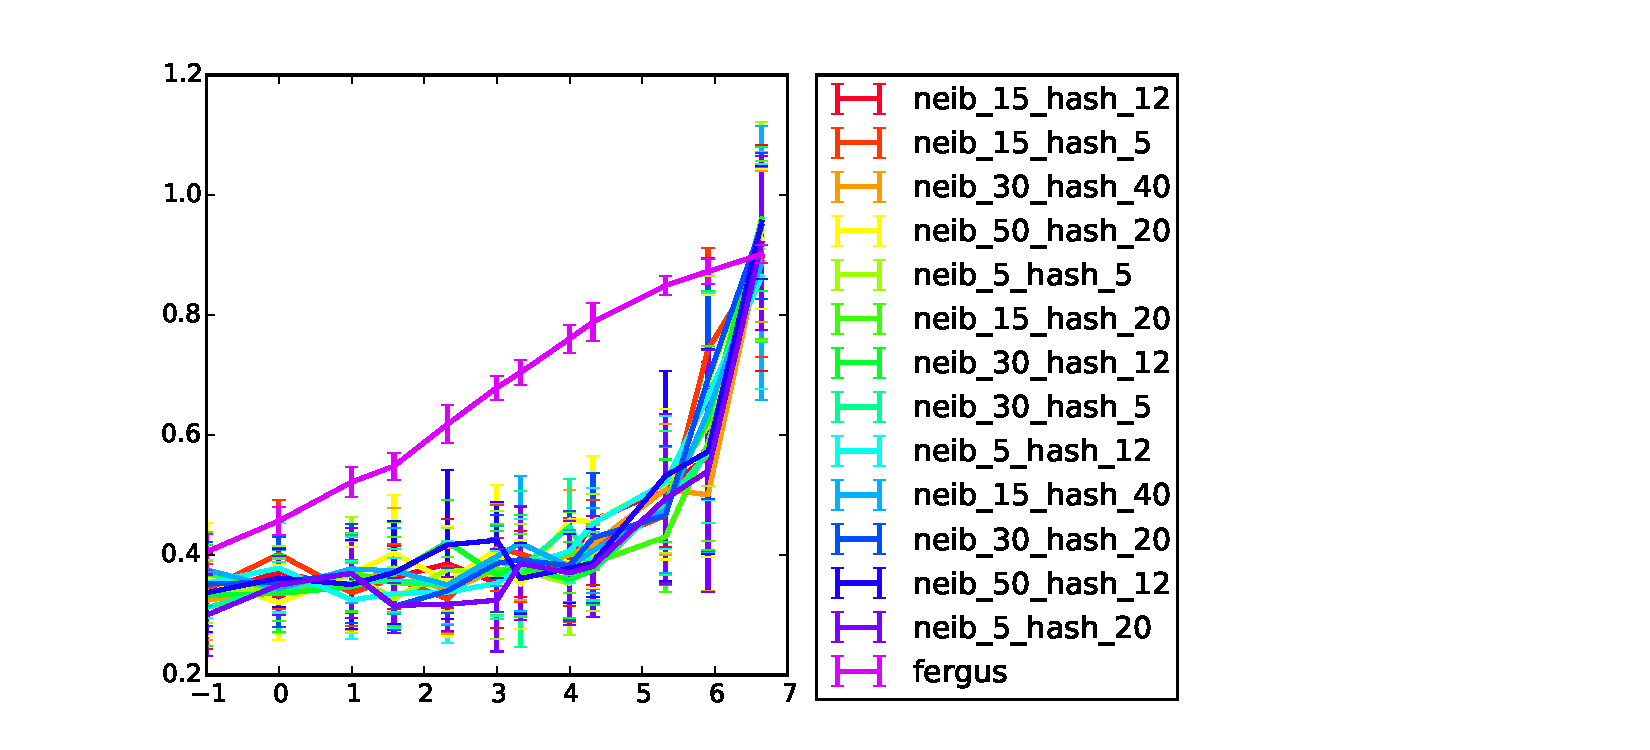
\includegraphics[width=1.8\textwidth]{method_comp.pdf}
\caption{Performance measures for different parameters}
\label{variation}
\end{figure}

We can see poor performance, barely better than random for low numbers of labeled points. Then, above 40 labeled positive points per class, performance increases significantly. We can assume that this lack of efficiency might be due to the reduction of the dataset, which certainly lowers the density of pointsand hence, the reliability of the ANN computation. This is also supported by the fact that values of parameters have little influence over performance.
\section{Conclusion and future work}

\end{document}
